\ifdefined\ishandout
  \documentclass[handout,landscape]{beamer} 
\else
  \documentclass[landscape]{beamer}
\fi

%\hypersetup{pdfpagemode=FullScreen} %Enabling this option will cause the slides to go full-screen on opening

\mode<handout>
{
  \usepackage{pgf}
  \usepackage{pgfpages}

\pgfpagesdeclarelayout{6 on 1 boxed}
{
  \edef\pgfpageoptionheight{\the\paperheight} 
  \edef\pgfpageoptionwidth{\the\paperwidth}
  \edef\pgfpageoptionborder{0pt}
}
{
  \pgfpagesphysicalpageoptions
  {%
    logical pages=6,%
    physical height=\pgfpageoptionheight,%
    physical width=\pgfpageoptionwidth%
  }
  \pgfpageslogicalpageoptions{1}
  {%
    border code=\pgfsetlinewidth{1pt}\pgfstroke,%
    border shrink=\pgfpageoptionborder,%
    resized width=.5\pgfphysicalwidth,%
    resized height=.5\pgfphysicalheight,%
    center=\pgfpoint{.25\pgfphysicalwidth}{.833\pgfphysicalheight}%
  }%
  \pgfpageslogicalpageoptions{2}
  {%
    border code=\pgfsetlinewidth{1pt}\pgfstroke,%
    border shrink=\pgfpageoptionborder,%
    resized width=.5\pgfphysicalwidth,%
    resized height=.5\pgfphysicalheight,%
    center=\pgfpoint{.75\pgfphysicalwidth}{.833\pgfphysicalheight}%
  }%
  \pgfpageslogicalpageoptions{3}
  {%
    border code=\pgfsetlinewidth{1pt}\pgfstroke,%
    border shrink=\pgfpageoptionborder,%
    resized width=.5\pgfphysicalwidth,%
    resized height=.5\pgfphysicalheight,%
    center=\pgfpoint{.25\pgfphysicalwidth}{.5\pgfphysicalheight}%
  }%
  \pgfpageslogicalpageoptions{4}
  {%
    border code=\pgfsetlinewidth{1pt}\pgfstroke,%
    border shrink=\pgfpageoptionborder,%
    resized width=.5\pgfphysicalwidth,%
    resized height=.5\pgfphysicalheight,%
    center=\pgfpoint{.75\pgfphysicalwidth}{.5\pgfphysicalheight}%
  }%
  \pgfpageslogicalpageoptions{5}
  {%
    border code=\pgfsetlinewidth{1pt}\pgfstroke,%
    border shrink=\pgfpageoptionborder,%
    resized width=.5\pgfphysicalwidth,%
    resized height=.5\pgfphysicalheight,%
    center=\pgfpoint{.25\pgfphysicalwidth}{.167\pgfphysicalheight}%
  }%
  \pgfpageslogicalpageoptions{6}
  {%
    border code=\pgfsetlinewidth{1pt}\pgfstroke,%
    border shrink=\pgfpageoptionborder,%
    resized width=.5\pgfphysicalwidth,%
    resized height=.5\pgfphysicalheight,%
    center=\pgfpoint{.75\pgfphysicalwidth}{.167\pgfphysicalheight}%
  }%
}


  \pgfpagesuselayout{6 on 1 boxed}[letterpaper, border shrink=5mm]
  \nofiles
}

\usepackage{listings}
\usepackage{multimedia}
\usepackage[normalem]{ulem}
\usepackage{ifthen}
\usepackage{textcomp}

\usetheme{Warsaw} 
\usecolortheme{seahorse}
\useoutertheme{infolines} 

\setbeamertemplate{blocks}[rounded][shadow=true] 

\author{Joe Fields}
\title{Introduction to Proof} 

\date{Lecture 29 (GIAM \S 6.1) \newline relations}
\institute[SCSU]{ {\tt fieldsj1@southernct.edu} }

\newcommand{\versionNum}{$3.2$\ }

\newboolean{InTextBook}
\setboolean{InTextBook}{false}
\newboolean{InWorkBook}
\setboolean{InWorkBook}{false}
\newboolean{InHints}
\setboolean{InHints}{false}

%When this boolean is true (beginning in Section 5.1) we will use the convention
% that $0 \in \Naturals$.  If it is false we will continue to count $1$ as the smallest
%natural number (thus making Giuseppe Peano spin in his grave...)
 
\newboolean{ZeroInNaturals}

%This boolean is used to distinguish the version where we use $\sim$ rather than $\lnot$

\newboolean{LNotIsSim}

%The values of the last two booleans are set in ``switches.tex''

\setboolean{ZeroInNaturals}{true}
\setboolean{LNotIsSim}{false}


\let\savedlnot\lnot
\ifthenelse{\boolean{LNotIsSim}}{\renewcommand{\lnot}{\sim} }{}

%This command puts different amounts of space depending on whether we are
% in the text, the workbook or the hints & solutions manual. 
\newcommand{\twsvspace}[3]{%
 \ifthenelse{\boolean{InTextBook} }{\vspace{#1}}{%
  \ifthenelse{\boolean{InWorkBook} }{\vspace{#2}}{%
   \ifthenelse{\boolean{InHints} }{\vspace{#3}}{} %
   }%
  }%
 }


\newcommand{\wbvfill}{\ifthenelse{\boolean{InWorkBook}}{\vfill}{}}
\newcommand{\wbitemsep}{\ifthenelse{\boolean{InWorkBook} }{\rule[-24pt]{0pt}{60pt}}{}}
\newcommand{\textbookpagebreak}{\ifthenelse{\boolean{InTextBook}}{\newpage}{}}
\newcommand{\workbookpagebreak}{\ifthenelse{\boolean{InWorkBook}}{\newpage}{}}
\newcommand{\hintspagebreak}{\ifthenelse{\boolean{InHints}}{\newpage}{}}

\newcommand{\hint}[1]{\ifthenelse{\boolean{InHints}}{ {\par \hspace{12pt} \color[rgb]{0,0,1} #1 } }{}}
\newcommand{\inlinehint}[1]{\ifthenelse{\boolean{InHints}}{ { \color[rgb]{0,0,1} #1 } }{}}

\newlength{\cwidth}
\newcommand{\cents}{\settowidth{\cwidth}{c}%
\divide\cwidth by2
\advance\cwidth by-.1pt
c\kern-\cwidth
\vrule width .1pt depth.2ex height1.2ex
\kern\cwidth}

\newcommand{\sageprompt}{ {\tt sage$>$} }
\newcommand{\tab}{\rule{20pt}{0pt}}
\newcommand{\blnk}{\rule{1.5pt}{0pt}\rule{.4pt}{1.2pt}\rule{9pt}{.4pt}\rule{.4pt}{1.2pt}\rule{1.5pt}{0pt}}
\newcommand{\suchthat}{\; \rule[-3pt]{.5pt}{13pt} \;}
\newcommand{\divides}{\!\mid\!}
\newcommand{\tdiv}{\; \mbox{div} \;}
\newcommand{\restrict}[2]{#1 \,\rule[-4pt]{.25pt}{14pt}_{\,#2}}
\newcommand{\lcm}[2]{\mbox{lcm} (#1, #2)}
\renewcommand{\gcd}[2]{\mbox{gcd} (#1, #2)}
\newcommand{\Naturals}{{\mathbb N}}
\newcommand{\Integers}{{\mathbb Z}}
\newcommand{\Znoneg}{{\mathbb Z}^{\mbox{\tiny noneg}}}
\ifthenelse{\boolean{ZeroInNaturals}}{%
  \newcommand{\Zplus}{{\mathbb Z}^+} }{%
  \newcommand{\Zplus}{{\mathbb N}} }
\newcommand{\Enoneg}{{\mathbb E}^{\mbox{\tiny noneg}}}
\newcommand{\Qnoneg}{{\mathbb Q}^{\mbox{\tiny noneg}}}
\newcommand{\Rnoneg}{{\mathbb R}^{\mbox{\tiny noneg}}}
\newcommand{\Rationals}{{\mathbb Q}}
\newcommand{\Reals}{{\mathbb R}}
\newcommand{\Complexes}{{\mathbb C}}
%\newcommand{\F2}{{\mathbb F}_{2}}
\newcommand{\relQ}{\mbox{\textsf Q}}
\newcommand{\relR}{\mbox{\textsf R}}
\newcommand{\nrelR}{\mbox{\raisebox{1pt}{$\not$}\rule{1pt}{0pt}{\textsf R}}}
\newcommand{\relS}{\mbox{\textsf S}}
\newcommand{\relA}{\mbox{\textsf A}}
\newcommand{\Dom}[1]{\mbox{Dom}(#1)}
\newcommand{\Cod}[1]{\mbox{Cod}(#1)}
\newcommand{\Rng}[1]{\mbox{Rng}(#1)}

\DeclareMathOperator\caret{\raisebox{1ex}{$\scriptstyle\wedge$}}

\newtheorem*{defi}{Definition}
\newtheorem*{exer}{Exercise}
\newtheorem{thm}{Theorem}[section]
\newtheorem*{thm*}{Theorem}
\newtheorem{lem}[thm]{Lemma}
\newtheorem*{lem*}{Lemma}
\newtheorem{cor}{Corollary}
\newtheorem{conj}{Conjecture}

\renewenvironment{proof}%
{\begin{quote} \emph{Proof:} }%
{\rule{0pt}{0pt} \newline \rule{0pt}{15pt} \hfill Q.E.D. \end{quote}}


\newcommand{\vs}{\rule{0pt}{11pt}}
\newcommand{\notimplies}{\;\not\!\!\!\implies}
\newcommand{\dx}{\,\mbox{d}x}

\AtBeginSection[]
{
 \begin{frame}{Table of Contents} 
  \tableofcontents[currentsection]
 \end{frame}
}

%%%% SAVE %%%%
%{ %magic to get a full screen image...
%\setbeamertemplate{navigation symbols}{}  % hide navigation buttons 
%\setbeamertemplate{background canvas}{\centerline{\includegraphics 
%	[height=\paperheight]{Cantor_4.jpeg}}}
%\begin{frame}[plain]
%\rule{0pt}{0pt}
%\end{frame} 
%} %end of magic


\begin{document}

\begin{frame}[plain]
  \titlepage
\end{frame}

\section{intro}

\begin{frame}{what is a relation?}
\begin{itemize}
\item Sometimes a symbol between two things means ``do an operation.'' \pause
\item Other times it means ``check a condition.'' \pause
\item Example: $3+4$ means ``add 3 and 4'' of course the answer is a number (7) \pause
\item Other example: $3=4$ means ``check if 3 and 4 are the same'' and here the answer is a boolean (FALSE).
\end{itemize}
\end{frame}

\begin{frame}{where is a relation?}
\begin{itemize}
\item Most of the relation symbols we know get numbers on both sides. \pause
\item $=$,  $\neq$, $<$, $\leq$, $>$, $\geq$ \pause
\item Some of the relation symbols we know get sets on either side \pause
\item $=$, $\subseteq$, $\supseteq$ \pause
\item One of the relation symbols we know gets different things on either side. \pause
\item $\in$
\end{itemize}
\end{frame}

\begin{frame}{an arrow diagram}
Here's a way to visualize the $\mid$ relation which is going {\em from} the set $\{1,2,3,6\}$ {\em to} itself. \pause

\begin{center}
\begin{picture}(0,0)%
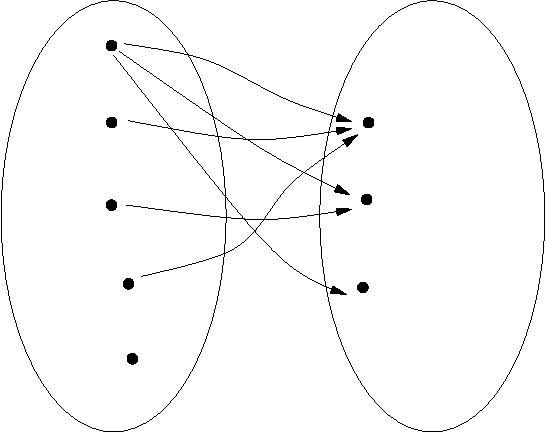
\includegraphics{figures/first_relation.pdf}%
\end{picture}%
\setlength{\unitlength}{3947sp}%
%
\begingroup\makeatletter\ifx\SetFigFont\undefined%
\gdef\SetFigFont#1#2#3#4#5{%
  \reset@font\fontsize{#1}{#2pt}%
  \fontfamily{#3}\fontseries{#4}\fontshape{#5}%
  \selectfont}%
\fi\endgroup%
\begin{picture}(4366,3466)(1193,-3819)
\put(1876,-811){\makebox(0,0)[lb]{\smash{{\SetFigFont{12}{14.4}{\familydefault}{\mddefault}{\updefault}{\color[rgb]{0,0,0}1}%
}}}}
\put(2026,-3286){\makebox(0,0)[lb]{\smash{{\SetFigFont{12}{14.4}{\familydefault}{\mddefault}{\updefault}{\color[rgb]{0,0,0}b}%
}}}}
\put(4276,-2011){\makebox(0,0)[lb]{\smash{{\SetFigFont{12}{14.4}{\familydefault}{\mddefault}{\updefault}{\color[rgb]{0,0,0}$\{1,3,5,7,\ldots\}$}%
}}}}
\put(4276,-1411){\makebox(0,0)[lb]{\smash{{\SetFigFont{12}{14.4}{\familydefault}{\mddefault}{\updefault}{\color[rgb]{0,0,0}$\{1,2,a\}$}%
}}}}
\put(4276,-2686){\makebox(0,0)[lb]{\smash{{\SetFigFont{12}{14.4}{\familydefault}{\mddefault}{\updefault}{\color[rgb]{0,0,0}$\{1\}$}%
}}}}
\put(2026,-2686){\makebox(0,0)[lb]{\smash{{\SetFigFont{12}{14.4}{\familydefault}{\mddefault}{\updefault}{\color[rgb]{0,0,0}a}%
}}}}
\put(1876,-1411){\makebox(0,0)[lb]{\smash{{\SetFigFont{12}{14.4}{\familydefault}{\mddefault}{\updefault}{\color[rgb]{0,0,0}2}%
}}}}
\put(1876,-2086){\makebox(0,0)[lb]{\smash{{\SetFigFont{12}{14.4}{\familydefault}{\mddefault}{\updefault}{\color[rgb]{0,0,0}3}%
}}}}
\end{picture}%

\end{center}   
\end{frame}

\begin{frame}{another arrow diagram}
Here's a way to visualize the $\in$ relation which is going {\em from} the set $\{1,2,3\}$ {\em to} its power set. \pause

\begin{center}
\begin{picture}(0,0)%
\includegraphics{first_relation-alt.pdf}%
\end{picture}%
\setlength{\unitlength}{3947sp}%
%
\begingroup\makeatletter\ifx\SetFigFont\undefined%
\gdef\SetFigFont#1#2#3#4#5{%
  \reset@font\fontsize{#1}{#2pt}%
  \fontfamily{#3}\fontseries{#4}\fontshape{#5}%
  \selectfont}%
\fi\endgroup%
\begin{picture}(4665,3166)(1193,-3144)
\put(1876,-811){\makebox(0,0)[lb]{\smash{{\SetFigFont{12}{14.4}{\familydefault}{\mddefault}{\updefault}{\color[rgb]{0,0,0}1}%
}}}}
\put(1876,-1411){\makebox(0,0)[lb]{\smash{{\SetFigFont{12}{14.4}{\familydefault}{\mddefault}{\updefault}{\color[rgb]{0,0,0}2}%
}}}}
\put(1876,-2086){\makebox(0,0)[lb]{\smash{{\SetFigFont{12}{14.4}{\familydefault}{\mddefault}{\updefault}{\color[rgb]{0,0,0}3}%
}}}}
\put(4426,-361){\makebox(0,0)[lb]{\smash{{\SetFigFont{12}{14.4}{\familydefault}{\mddefault}{\updefault}{\color[rgb]{0,0,0}$\emptyset$}%
}}}}
\put(4426,-661){\makebox(0,0)[lb]{\smash{{\SetFigFont{12}{14.4}{\familydefault}{\mddefault}{\updefault}{\color[rgb]{0,0,0}$\{1\}$}%
}}}}
\put(4426,-1036){\makebox(0,0)[lb]{\smash{{\SetFigFont{12}{14.4}{\familydefault}{\mddefault}{\updefault}{\color[rgb]{0,0,0}$\{2\}$}%
}}}}
\put(4426,-1411){\makebox(0,0)[lb]{\smash{{\SetFigFont{12}{14.4}{\familydefault}{\mddefault}{\updefault}{\color[rgb]{0,0,0}$\{3\}$}%
}}}}
\put(4426,-1786){\makebox(0,0)[lb]{\smash{{\SetFigFont{12}{14.4}{\familydefault}{\mddefault}{\updefault}{\color[rgb]{0,0,0}$\{1, 2\}$}%
}}}}
\put(4426,-2161){\makebox(0,0)[lb]{\smash{{\SetFigFont{12}{14.4}{\familydefault}{\mddefault}{\updefault}{\color[rgb]{0,0,0}$\{1, 3\}$}%
}}}}
\put(4426,-2536){\makebox(0,0)[lb]{\smash{{\SetFigFont{12}{14.4}{\familydefault}{\mddefault}{\updefault}{\color[rgb]{0,0,0}$\{2, 3\}$}%
}}}}
\put(4426,-2911){\makebox(0,0)[lb]{\smash{{\SetFigFont{12}{14.4}{\familydefault}{\mddefault}{\updefault}{\color[rgb]{0,0,0}$\{1, 2, 3\}$}%
}}}}
\end{picture}%

\end{center}   
\end{frame}


\begin{frame}{who is a relation}
\begin{itemize}
\item Remember the roster form for a set? \pause
\item Some would say that the best way to describe a set is to give its roster form. \pause
\item In the same spirit, how can we best describe a relation? \pause
\item Fundamentally, the identity of a relation is tied to the set of ordered pairs that make it true.\pause
\item So, for example, the relation where we were looking at the divisors of 6 might best be represented by the following set: \pause

\[ \{ (1,1), (1,2), (1,3), (1,6), (2,2), (2,6), (3,3), (3,6), (6,6) \} \]

\end{itemize}
\end{frame}

\section{Cartesian products}

\begin{frame}{cogito ergo sum}
\begin{itemize}
\item Since relations are best understood as sets of ordered pairs \pause
\item we need to know about ordered pairs. \pause
\item The $x-y$ plane may be the best exemplar. \pause
\item A digression about Ren\'{e} DesCartes\textellipsis
\end{itemize}
\end{frame}

\begin{frame}{Artoo}
\begin{itemize}
\item $\displaystyle A \times B \; = \; \{ (a,b) \suchthat a \in A \, \land \, b \in B \} $ \pause
\item The special case where $A = B = \Reals$ is the Cartesian plane
\item By analogy with ordinary multiplication we get a way to interpret powers of a set. \pause
\item $\displaystyle \Reals^2 \, = \, \Reals \times \Reals$ \pause
\item $\displaystyle \Reals^3 \, = \, \Reals \times \Reals \times \Reals$ \pause
\item Anyway, the generic deal is that {\em any} subset of a Cartesian product is a relation.
\end{itemize}
\end{frame}

\section{notation}

\begin{frame}{the fix is in}
\begin{itemize}
\item We use infix notation (stick the relation symbol in between its arguments) \pause
\item When we're dealing with an abstract relation on a set $S$ it is just a subset of $S^2$. \pause
\item $\displaystyle  \relR \, \subseteq \, S \times S$. \pause
\item Just treat the name of the relation just like it was a $<$ sign! \pause
\item So $a \relR b$ just means that $(a,b)$ is one of the pairs in $\relR$.
\end{itemize}
\end{frame}

\begin{frame}{a special case}
\begin{itemize}
\item Functions are just relations that satisfy an additional property. \pause \newline
(Basically, the vertical line test.) \pause
\item Suppose $f$ is a function. \pause
(A real-valued function of a real variable.) \pause
\item We could presumably write $xfy$ to mean that $x$ gets mapped to $y$ by the function $f$. \pause
\item Nobody does that! \pause
\item For functions we use Euler notation rather than infix notation. \pause
\item $y = f(x)$ is the the same thing as saying the pair $(x,y)$ is in the relation $f$.

\end{itemize}
\end{frame}


\section{composition and inverses}

\begin{frame}{}
\begin{itemize}
\item There are a couple of operations you are certainly familiar with in the ``functions'' setting:\pause
\item Composition and Inverses. \pause
\item Composition -- Like hooking $\sqrt{x}$ and $3x+1$ together to get $\sqrt{3x+1}$. \pause \newline
Or, $3\sqrt{x}+1$ if you do it other way around\textellipsis \pause 
\item Inverses -- Like how $e^x$ and $\ln{(x)}$ undo one another. \pause
\item These make sense for relations too.
\end{itemize}
\end{frame}

\begin{frame}{switching things around}
\begin{itemize}
\item Consider the input/output pairs that happen when $f$ and its inverse $f^{-1}$ are applied to numbers. \pause
\item If $f(a) = b$ then $f^{-1}(b) = a$.  \pause And vice versa. \pause
\item If we we-write that using infix notation we get 
\[ afb \, \iff \, bf^{-1}a. \] \pause
\item This gives us a hint how the inverse of an arbitrary relation should work. \newline
Here are two versions: \pause
\item $\displaystyle a \relR b \, \iff b \, \relR^{-1} a$ \pause

\centerline{or,} \pause

\item $\displaystyle \relR^{-1} \, = \, \{ (b,a) \suchthat (a,b) \in \relR \}$ \pause
\end{itemize}
\end{frame}

\begin{frame}{hooking things up}
\begin{itemize}
\item When you compose two functions, say $f(g(x))$, you need to first compute $g(x)$ \pause \newline
{\em then} apply $f$ to that intermediate result. \pause
\item To compose two relations, we focus on this idea of the ``intermediate result.'' \pause
\item The picture to keep in your mind's eye is: \pause

\begin{center}
\input{comp_of_rels.tex}
\end{center}

\end{itemize}
\end{frame}

\begin{frame}{composition}
\begin{itemize}
\item Be mindful of the reversal of order!\pause
\item $\relR$ is a relation from $A$ to $B$, and $\relS$ is a relation from $B$ to $C$. \pause
\item (Alternatively, we might say $\relR \subseteq A \times B$ and $\relS \subseteq B \times C$.) \pause
\item The composition goes from $A$ to $C$. \pause
\item Is the thing we've been picturing $\relR \circ \relS$ or is it $\relS \circ \relR$? \pause
\item Again, think back to the function notation. \pause \newline
$f \circ g (x) \; = \; f(g(x))$ and, written in that order, it is $g$ that is applied first to $x$. \pause
\item The composition of relations we've been looking at has $\relR$ first, so it is written $\relS \circ \relR$. \pause
\item Danger!
\end{itemize}
\end{frame}

\begin{frame}{composition 2}
\begin{itemize}
\item Alright! So. Most of the time (all of the time in GIAM) we read compositions right-to-left.\pause
\item Here's the formal definition: \pause

Suppose $\relR$ is a relation from $A$ to $B$ and $\relS$ is a relation from $B$ to $C$, then $\relS \circ \relR$ is a relation from $A$ to $C$ defined by \pause

\[ \relS \circ \relR \; = \; \{ (a,c) \in \, A \times C \, \suchthat \; \exists b \in B, \; (a,b) \in \relR \; \land \; (b,c) \in \relS \}. \]
\pause

\item You may also express the same thing using infix notation: \pause

\[ a(S\circ R)c \; \iff \; \exists b \in B, \; a\relR b \; \land \; b\relS c.\]

\end{itemize}
\end{frame}
\end{document}
